\section{Exercise 1: Find instances of Design Patterns}

In this exercise, we had to find instances of design patterns in jEdit's
code, jEdit being an open source text editor written in Java.

\subsection{Singleton}

The singleton pattern is categorized as a creational pattern because it
ensures that a specific class is \textbf{instantiated} only once.\\

It is often criticized because an instance of a class using this pattern
can be used like a global variable. A global variable causes problem for
unit testing, because it can be modified by everyone and causes
unpredictability in the state of the system. It also introduces coupling
with classes using it, which renders them hardly reusable.\\

While using global variables may be seen as bad practice, and while
there are alternatives (e.g. dependency injection), these alternatives
may bring drawbacks such as having the code difficult to read, or the
intent of the developpers may not be easy to grasp at first glance.
Global variables may even be the simplest way of using tools such as a
Logging classes which is not directly part of the application but only
here to help debugging.\\

The example we chose for a singleton implementation is the
\emph{PluginManager}\footnote{\emph{org.gjt.sp.jedit.pluginmgr} package}
class. This class handles the window (extends \emph{JFrame}) where
plugins are installed and updated. The singleton pattern is used in this
case so that only one plugin manager window can be instantiated and
displayed at once when invoking it via the menu (\emph{Plugins -> Plugin
Manager...}). The following methods are involved :

\begin{itemize}\itemsep1pt
    \item the \emph{showPluginManager()} method instantiate a PluginManager if
    it has not already been instantiated, else it brings the plugin manager
    window to the front;

    \item The \emph{getInstance()} method retrieve the current instance of
    PluginManager (can be null if it has not yet been instantiated or if
    the instance has been disposed of with the \emph{dispose()} method).
\end{itemize}

\begin{figure}[h!]
    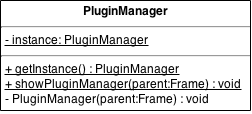
\includegraphics[width=0.4\textwidth]{images/singleton.png}
    \centering
    \caption{Singleton example class diagram}
\end{figure}

\begin{framehint}
    The following classes are also implementing a singleton pattern, but they
    will not be described in details.

    \begin{itemize}\itemsep1pt
        \item \emph{ReflectManager} (\emph{org.gjt.sp.jedit.bsh})
        \item \emph{KillRing} (\emph{org.gjt.sp.jedit.buffer})
        \item \emph{ModeProvider} (\emph{org.gjt.sp.jedit.syntax})
        \item \emph{TransferHandler} (\emph{org.gjt.sp.jedit.datatransfer})
        \item \emph{DockableWindowFactory} (\emph{org.gjt.sp.jedit.gui})
    \end{itemize}
\end{framehint}
\newpage

\subsection{Abstract Factory}

\noindent The abstract factory pattern is a creational pattern which helps creating
related objects.\\

The example found in jEdit's code is centered around the
\emph{StatusWidgetFactory} interface which must be implemented by all the
factories related to constructing statusbar widgets. Examples of factories
implementing it are \emph{ErrorsWidgetFactory}, \emph{ClockWidgetFactory},
\emph{LastModifiedWidgetFactory}. Its purpose is to instantiate StatusBar
widgets without having to specify the concrete class needed to construct it.

\begin{figure}[h!]
    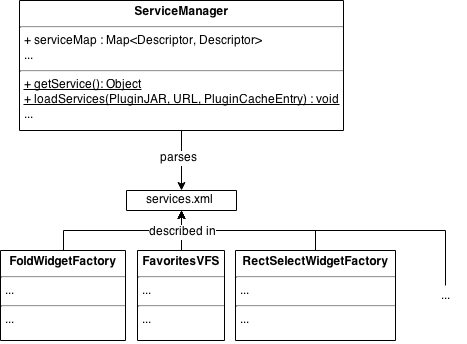
\includegraphics[width=0.8\textwidth]{images/abstractfactory.png}
    \centering
    \caption{Abstract Factory example class diagram}
\end{figure}

\begin{framehint2}
\textbf{N.B.} Statusbar widgets also seem to be used as services and are listed
in the \emph{services.xml} file. This file specifies the services' classes or
factory classes, names and ways of instantiating them (constructor to call).
Each service is a singleton handled by the \emph{ServiceManager}.
By loading services through an XML file, the program handles the
instantiation of services the same way for all services. Furthermore, the
program's code does not need to be modified to add a service, only the
xml must be modified; hence, the \emph{ServiceManager} does not need to
depend on all the services' factories and the coupling is reduced.
\end{framehint2}
\newpage

\subsection{Observer}

\subsection{Adapter}

\subsection{Visitor}

\newpage
